% It is an example file showing how to use the 'acm_proc_article-sp.cls' V3.2SP
% LaTeX2e document class file for Conference Proceedings submissions.
\documentclass{edm_template}

\usepackage{graphics}

\begin{document}

\title{Measuring the moment of learning with an information-theoretic approach}
\numberofauthors{1}
\author{
\alignauthor
      Brett van de Sande\\
       \affaddr{Arizona State University}\\
       \affaddr{PO Box 878809}\\
       \affaddr{Tempe, AZ~~85287}\\
       \email{bvds@asu.edu}
}

\maketitle
\begin{abstract}
There are various methods for determining the moment at which a
student has learned a given skill.  Using the Akaike information
criterion (AIC), we introduce an approach for determining the
probability that an individual student has learned a given skill at a
particular problem-solving step.  We then investigate how well this
approach works when applied to student log data.  Using log data from
students using the Andes intelligent tutor system for an entire
semester, we show that our method can detect statistically significant
amounts of learning, when aggregated over skills or students.  In the
context of intelligent tutor systems, one can use this method to
detect when students may have learned a skill and, from this
information, infer the relative effectiveness of any help given to the
student or of any behavior in which the student has engaged.
\end{abstract}

\keywords{data mining, models of student learning}


\section{Introduction}

%
%  There is a post-it with note''  ``ICAP frame chi Cog Sci''
%  http://gamesandimpact.org/uncategorized/cgi-qa-with-asu-fellow-dr-michelene-micki-chi/
%

%Talk about ultimate goal of using this to determine effectiveness
%of help given or of a particular student behavior.

The traditional experimental paradigm for studying student learning
is to use a pre-test and post-test combined with two or more experimental
conditions.  Pre-test and post-test scores can indicate {\em whether}
learning has occurred, but not {\em when} it may have occurred.  
At best, one might infer when learning has occurred if an isolated change to 
the instructional materials or help-giving strategy results in better
post-test performance.  
It is more difficult to infer whether a change in student {\em behavior} at
some point has resulted in greater learning, since student behavior is 
largely uncontrolled and must be recorded in some way.
In a laboratory setting, these issues can be addressed by careful
experimental design, albeit with an accompanying loss of authenticity.

Moving from the laboratory to a more realistic setting, such as a
classroom study, presents as challenge since there is necessarily an
extended time between any pre-test and post-test.  Heckler and 
Sayre~\citeyear{heckler_what_2010} introduce an experimental technique
where they administered a test to a different subgroup of students in
a large physics class each week during the quarter, cycling through
the entire class over the course of the quarter (a
between-students longitudinal study).  With a sufficiently large number
of students (1694 students over five quarters), they were able to produce
plots of student mastery of various skills as a function of time, and
identify exactly which week(s) students learned a particular skill.
However, the shortest time scale that one could imagine for this
kind of approach (administering a test in a classroom setting) can, at
best, be a day or so.  Can we do better?

The use of an intelligent tutor systems (ITS) provides a way forward. 
An ITS is a computer-based learning environment where students
construct problem solutions on a user interface and the system
evaluates the student work at the step-level. 
Examples include the CMU LISP tutor~\cite{corbett_knowledge_1995}, the
Carnegie Learning Cognitive Tutors~\cite{koedinger_illustrating_1998},
and Andes~\cite{vanlehn_andes_2005}.  In these tutors, student
activity is analyzed and logged for each user interface element change, with a granularity
of typically several 10s of seconds.
Instead of relying on a distant pre-test or post-test, the experimenter can examine student
(or tutor system) activity in the immediate vicinity of the event of interest.

Our stated goal is to determine student learning for an individual
student as they progress through a course.  What observable quantities should be used to
determine student mastery?  One possible observable is ``correct/incorrect steps,''  whether 
the student correctly applies a given skill at a particular problem-solving step 
without any preceeding errors or hints.  There are other
observables that may give us clues on mastery: for instance, how much
time a student takes to complete a step that involved a given skill.  However, other such
observables typically need some additional theoretical interpretation. {\em Exempli gratia},
What is the relation between time taken and mastery?  Baker, Goldstein, and
Heffernan~\citeyear{baker_detecting_2011} develop a model of learning
based on a Hidden Markov model approach.  They start with a set of
% BvdS:  use actual number.
25 additional observables (including ``time to
complete a step'') and construct their model and use correct/incorrect steps (as defined above)
to calibrate the additional observables and determine which are significant.

Since correct/incorrect steps is easy to interpret, we will use that
as the starting point for our investigation.  Naturally, it is
desirable to eventually include various other observables in any determination
of student learning.

To start our investigation, we will compare three different models of
learning using data from students taking introductory physics and examine
whether there is empirical support for using one model over the
others.  In fact, using Akaike Information Criteria (AIC), we obtain
results that seem to favor two models over the third, but note
that fitting the models to individual students can make the determination ambiguous.

Second, we introduce a multi-model approach to predict the probability that 
learning has occurred at a given step, and how much
learning has occurred.  We apply our approach to student log data from
and introductory physics course and discuss the reliability of any
predictions of skill mastery.  We find that, for an individual
student and skill, detection of learning has large uncertainties.
However, if one aggregates over skills or students, then learning can
be detected at the desired level of significance.


\subsection{Correct/Incorrect steps}

As mentioned above, we will use correctness/incorrectness of a step to
determine when the student has learned above.  Thus, we need to
define precisely what we mean by a step being correct.

A student attempts some number of {\em steps}  when solving a problem.  
Usually, a step is associated with creating/modifying a single user
interface object (writing an equation, drawing a vector,
defining a quantity, {\em et cetera}) and is a distinct part of the problem solution
(that is, help-giving dialogs are not considered to be steps).
A student may attempt a particular problem solving
step, delete the object, and later attempt that solution step again.
A step is an {\em opportunity} to learn
a given  Knowledge Component (KC)~\cite{vanlehn_behavior_2006} if the student 
must apply that skill to complete the step.

%
%  Not needed in this paper.
%
%Each step $j$ corresponds some some number of student-tutor 
%{\em transactions}: attempts at constructing the associated object, 
%or associated interactions with the Andes help system.  

%Next, we need a model of student learning for a particular KC.
%Since the policies chosen by the random-help version of Andes
%are different for each student,
%we need to determine the point of learning for each student.
For each KC and student, we select all attempted steps that involve application
of that KC and mark each step as ``correct'' if
the student completes that step correctly without any preceeding errors or 
requests for help; otherwise, we mark the step as ``incorrect.''
\label{steps}  % Section reference for correct/incorrect
If each incorrect/correct step is marked with a 0/1, then
a single student's performance on a single KC can be expressed as a bit  sequence,
{\em exempli gratia} 00101011.  We will label
steps with $j\in\left\{1,\ldots,n\right\}$.  

\section{The step model}

\begin{figure}
  \centering \includegraphics{step-model.eps}
  \caption{Functional form of the three models of student learning.}
    \label{step-model}
\end{figure}

\subsection{Method}


\begin{figure}
  \centering 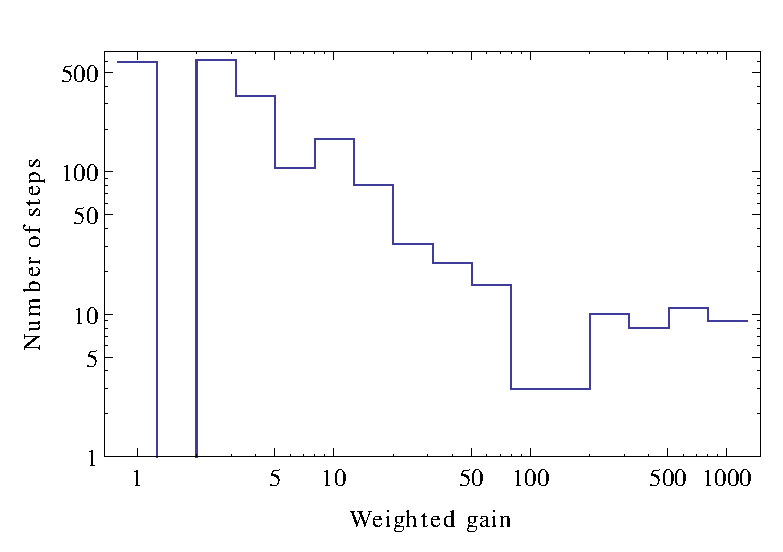
\includegraphics{student-kc-length-histogram.eps}
  \caption{Histogram of number of distinct student-KC sequences in student 
    dataset $\mathcal{A}$ having a given number of steps $n$.}
    \label{student-length-histogram}
\end{figure}

We examined log data from 12 students taking an intensive introductory
physics course at St.\ Anselm College during summer 2011.  The course
covered the same content as a normal two-semester introductory course.
Log data was recorded as students solved homework problems while using
the Andes intelligent tutor homework system.  231 hours of log data
were recorded.
%, covering 85,744 transactions, and 26,204 student steps.  
Each step was assigned to one or more different KC's.  The dataset
contains a total of 2017 distinct student-KC sequences covering a total of
245 distinct KC's.  We will refer to this dataset as student dataset
$\mathcal{A}$.  See Figure~\ref{student-length-histogram} for a
histogram of the number student-KC sequences having a given number of
steps.

Most KC's are associated with physics
or relevant math skills while others are associated with 
Andes conventions or user-interface actions (such as, notation
for defining a variable).  The student-KC sequences with the largest 
number of steps are associated with user-interface related skills,
since these skills are exercised throughout the entire course. 

One of the most remarkable properties of the distribution in
Fig.~\ref{student-length-histogram} is the large number of
student-KC sequences containing just a few steps.
The presence of many student-KC sequences with just one or two
steps may indicate that the default cognitive model associated 
with this tutor system may be sub-optimal; to date, there has not 
been any attempt, to date, to improve on the cognitive model of 
Andes with, say, Learning Factors Analysis~\cite{cen_learning_2006}.
Another contributing factor is the way that introductory physics is 
taught in most institutions, with relatively little repetition of 
similar problems.  This is quite different than, for instance, 
a typical middle school math curriculum where there are a large number
of similar problems in a homework assignment.



\section{Multi-model approach}
\label{multi-model}

We need to determine the step where a specific student has learned a
particular skill.  Our strategy is to take the step model, 
$P_\mathrm{step}(j)$, and treat $L$ as a constant, yielding a set of $n$ 
sub-models $P_{\mathrm{step},L}(j)$, one for each value of $L$.
We then fit each of the $n$ sub-models to the student data and
calculate an AIC value.  Finally, we find the Akaike weighs for each of the
sub-models.  The Akaike weights give the relative probability that learning
occurred at each step.

\begin{figure}
  \centering \includegraphics{step-weights.eps}
   \caption{Akaike weights for the submodels $P_\mathrm{step,L}(j)$.  
     This gives the relative probability that
      the student learned the KC just before step $L$.}
    \label{step-weights}
\end{figure}

Let us illustrate this technique with a simple example.  Suppose the
bit sequence for a particular student-KC sequence is 00011011 (8
opportunities); see Fig.~\ref{step-weights}.  We fit this bit sequence to 8
sub-models of the step model, corresponding to $L\in\{1,2,\ldots,8\}$,
by maximizing the log likelihood $\log\mathcal{L}$.  The associated
AIC values are given by $\mathrm{AIC}_L=2 K-\log \mathcal{L}$ where
$K$ is the number of fit parameters.  Note that there are two
parameters ($s$ and $g$) when $L>1$ and there is only one parameter
($s$) when $L=1$.
%
%\begin{table}
%\caption{
%\begin{tabular}{crrrrrrrr}
% opportunity & 1 & 2 & 3 &4 & 5 & 6 & 7 & 8 \\
 % AIC &   13.1 & 13.6 & 11.6 & 9.0 & 13.0 & 14.5 & 11.6 & 13.6 \\
%\end{tabular}
%\end{equation}
%
Not surprisingly, the best fit (lowest AIC) corresponds to the first
``1'' in the bit sequence at step~4.  From the AICs, we calculate 
the Akaike weights
%
\begin{equation}
     w_L=\frac{e^{-\mathrm{AIC}_L/2} }{\sum_{L^\prime}
       e^{-\mathrm{AIC}_{L^\prime}/2}} \; .
\end{equation}
%
The Akaike weight $w_L$ gives the relative probability that sub-model 
$P_{\mathrm{step},L}(j)$ is, of all the sub-models, the closest to the 
the model that actually generated the data.


Note that the case $L=1$ corresponds to the student having 
``learned the skill'' some time before the first step.  That is to say, 
the student does not acquire the skill while using the tutor system.
Thus, $w_1$ should be interpreted as the relative probability
that no learning has occurred while using the tutor system.

\section{Weighted gain}

Our ultimate goal is to distinguish steps that result in 
learning from steps that do not.  Hopefully, one can use this
information to infer something about the effectiveness of the help
given on a particular step, or the effectiveness of
the student activity on that step.

\begin{figure}
  \centering \includegraphics{weighted-gain-histogram.eps}
   \caption{Histogram of weighted gains $w_L \Delta_L$ for
     all steps in all student-KC sequences in student dataset $\mathcal{A}$.}
    \label{weighted-gain-histogram}
\end{figure}

It is not sufficient to know {\it when} learning has occurred but one
must also determine {\it how much} learning has occurred.  Consider
the bit sequence 11011000.  When fit to the step model, the best fit
will occur at $L=6$ but this would correspond to a {\it decrease} in student
performance for that skill.  In many cases seen in our log data, 
the change in student performance is almost zero.  In order to take 
this into account,
we propose using the Akaike weight $w_L$ times the associated learning
gain $\Delta_L$ to characterize a step.  We define the learning gain
$\Delta_L=1-\hat{g}-\hat{s}$ where $\hat{g}$ and $\hat{s}$ are the
Maximum Likelihood estimators for $g$ and $s$ given by submodel
$P_{\mathrm{step},L}(j)$.  For the ``no learning'' case $L=1$, we set
$\Delta_1=0$.  We will call $w_L \Delta_L$ the ``weighted gain''
associated with $P_{\mathrm{step},L}(j)$.  A histogram of $w_L
\Delta_L$ for student dataset $\mathcal{A}$ is shown in
Fig.~\ref{weighted-gain-histogram}.  Note that the vast majority of
steps (29730) have almost zero weighted gain.  We also see that there
is a significant number of steps with negative gain (988), but there
are somewhat more steps with positive gain (1312) .

The fact that there are so many steps with negative gain is
symptomatic of bit sequences that are very noisy (a lot of
randomness).  Indeed, if we compare the histogram for student
dataset $\mathcal{A}$ with the histogram for a randomly 
generated dataset $\mathcal{R}$ (we take $\mathcal{A}$ and
randomly permute the steps) we find a similar distribution;
see Fig.~\ref{weighted-gain-histogram2}.

What would the distribution look like if the data weren't 
so noisy?  To see this, we generated an artificial ``ideal'' dataset
$\mathcal{I}$ where there were no slips or guesses, but having
the same length distribution as $\mathcal{A}$ 
(Fig.~\ref{student-length-histogram}).  Thus, the bit sequences
in $\mathcal{I}$ have the form $00\cdots011\cdots1$.
In this case, for each student-KC sequence, we expect a single 
large weighted gain (corresponding to the first 1 in the bit sequence) 
and the remaining weighted gains to be nearly zero.  The resulting 
distribution of gains is shown
in  Fig.~\ref{weighted-gain-histogram2}.

\begin{figure}
  \centering 
\includegraphics{weighted-gain-histogram2.eps}
   \caption{Histogram of weighted gains $w_L \Delta_L$ for
     the student dataset $\mathcal{A}$, 
     a randomly generated dataset $\mathcal{R}$,
     and an artificial ideal dataset $\mathcal{I}$.}
    \label{weighted-gain-histogram2}
\end{figure}


We propose to use the following average of the weighed gains as
a ``quality index'' for determining how suitable a 
dataset is for determining the point of learning for an individual
student-KC sequence:
%
\begin{equation}
           Q= \frac{1}{N} \sum_\alpha \sum_L w_L \Delta_L
\end{equation}
%
where $\alpha$ is an index running over all student-KC sequences in a 
dataset and $N$ is the number of student-KC sequences.
We use the sample standard deviation of the weighted gains $w_L \Delta_L$
to calculate the standard error associated with $Q$. 

For the random dataset $\mathcal{R}$, the distribution of $\Delta_L$
is symmetric about zero and $Q$ approaches zero as $N \to \infty$.
For the ``ideal'' dataset $\mathcal{I}$, we expect, for the first 1 in
the bit sequence, $w_L$ to be nearly one with the associated $\Delta_L$
also nearly one so that $Q\to 1$ in the limit of many opportunities.
Numerically, we obtain $Q=0.5240\pm0.0003$.  The fact that it is
smaller than one is due to the large number of student-KC sequences having
just a few steps.  For the student dataset $\mathcal{A}$, we obtain
$Q=0.0467\pm0.0065$, which is small, but significant
($p<0.001$). Thus, we conclude that this student dataset is of
sufficient quality to use in determining where learning has occurred.


\section{Conclusion}

We believe that a direct estimate of the moment when a student
learns a skill could be very useful for improving instruction,
improving help-giving and understanding student learning.
However, the question of whether learning has occurred at a particular
step can only be answered in a probabilistic sense:
unambiguous ``Aha moments'' seem to be relatively rare.
Using the Akaike Information Criterion, we have introduced a method
for determining this probability.



As can be seen in
Fig.~\ref{weighted-gain-histogram2}, there is not much difference
between a student dataset and a randomly generated dataset.  However,
the quality index $Q$ which can be used to quantify the
size of the signal as well as the size of the background.  We see that
$Q=0.0467\pm0.0065$ for the student dataset $\mathcal{A}$ is roughly
10\% the size of $Q$ for the ideal dataset $\mathcal{I}$; we interpret
this to mean that the ``signal'' is roughly 10\% as big as the
``noise.''  However, the fact that $Q$ for the student dataset is
seven standard deviations from zero means that we have detected
learning for 2000 student-KC sequences with room to spare.  Using the fact
that the error goes as $1/\sqrt{N}$, where $N$ is the number 
of student-KC sequences, we estimate
that we could still detect learning with only 260 student-KC sequences at the
$p=0.01$ level.  This gives us an initial estimate for the amount of
log data needed to measure the moment of learning, at least for
students using the Andes tutor system.

As seen in Fig.~\ref{student-length-histogram}, we see that many of
the student-KC sequences are quite short.  We speculate that this
is due to to the way that physics is typically taught, with relatively
little reinforcement of specific KCs, emphasizing, instead, more
general problem solving meta-skills.  If we were to repeat this
analysis for high school or grade school math, where there is more
repetition, we speculate that there would be significantly fewer KCs
with less than 10 opportunities and that detecting when learning has
occurred would be significantly easier.


%ACKNOWLEDGMENTS are optional
\section{Acknowledgments}
Funding for this research was provided by the Pittsburgh Science of
Learning Center which is funded by the National Science Foundation
award No. SBE-0836012.

%
% The following two commands are all you need in the
% initial runs of your .tex file to
% produce the bibliography for the citations in your paper.
\bibliographystyle{abbrv}
\bibliography{education-modeling}
%Generated by bibtex from your ~.bib file.  Run latex,
%then bibtex, then latex twice (to resolve references)
%to create the ~.bbl file.  Insert that ~.bbl file into
%the .tex source file and comment out
%the command \texttt{{\char'134}thebibliography}.

\end{document}
